\chapter{Measurement technology for laser-camera triangulation}
\label{ch:technology}
%
% Original title:
%  La tecnologia di misura per la triangolazione laser-telecamera
%

\textit{In this chapter we will introduce the laser-camera triangulation technology, with particular attention to its details, components and problems. We will also present the camera calibration problem and conclude with a comparison with the main stereo vision technologies.}

% The laser-camera triangulation technology
  \section{Laser-camera triangulation technology}
\label{sec:lctt}
In computer vision, the term \textit{triangulation} refers to the ability to determine a 3D point in the world, through its projections in two or more image planes. Usually the expression ``laser triangulation'' has become a synonym for a system that measures distances using a sensor and a laser. In this thesis, the terms \textit{laser triangulation}, ``\textit{Sheet Of Light}'' (\acs{SOL}), or \textit{light stripe triangulation} will be used as synonyms even though this is not entirely correct, because of the type of laser projector used. Afterwords we will consider only laser stripes. \\

In a 3D triangulation system the three main components are:
\begin{itemize}
  \item a camera (typically based on CCD or C-MOS sensors);
  \item a laser projector (typically a collimated laser);
  \item a software to process images and accurately translate pixel offsets to height differences.
\end{itemize}
In this systems a laser beam is projected against a target object, while one or more acquisition sensors collect images of scene, as in Figure \ref{fig::triang_config}. The analysis of the laser shape on the images allows to reconstruct the object and make measures on it.
\begin{figure}[t!]
  \centering
  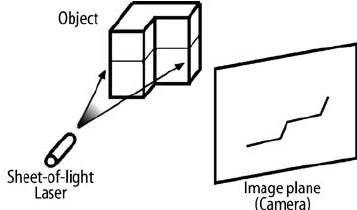
\includegraphics[width=0.5\textwidth]{./images/tech/triang_model_2.png}
  \caption{Example of laser-camera triangulation system}
  \label{fig::triang_config}
\end{figure} \\
Camera and laser are fixed each other and, at the same time, they are rotated at a known angle. In Figure \ref{fig::triang_geoms} the most common system configurations are shown. Each of them has its own pros and cons. \\

\begin{figure}[!b]
  \centering
  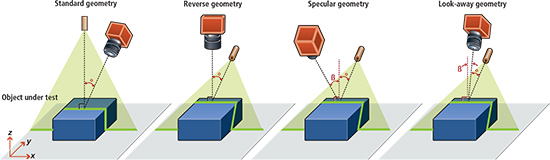
\includegraphics[width=\textwidth]{./images/tech/tech_geometry.jpg}
  \caption{Typical laser-camera configurations}
  \label{fig::triang_geoms}
\end{figure}

\noindent
In the \textit{standard geometry}, the laser line is projected perpendicularly to the $\left( x, y \right)$ nominal plane. This is the simplest configuration because the variation in the target height does not change the coordinate $y$ in the nominal plane. If on the one hand this simplifies system calibration and target shape analysis, resulting in a very fast and accurate system, on the other the camera views the object from a corner by changing the depth of field of the camera. The accommodation of the camera is needed, in order to keep the focus at the height of the object, moreover a test object must be calibrated for accurate measurement results from the system. \\

\noindent
If we switch the positions of projector and camera, we produce the \textit{reverse geometry}. In this case the system is more sensitive to the change in the height of the target, because the laser inclination causes a large shift in the position of the laser line. However these shifts change the value of the $y$ coordinate in the nominal plane, causing a more complex analysis.\\

\noindent
In \textit{specular geometry} configurations, both the projector and camera are placed at non-normal angles compared to the target surface. The placement allows a greater height resolution than the previous configurations, but the camera could see laser specular reflections. This causes noisy effect when acquiring images, such as saturation or blooming. As it happened in reverse geometry, laser inclination caused changes in $y$ coordinates when varying the height of the object. \\

\noindent
The \textit{look-away geometry} was introduced to reduce the laser specular reflections, by placing the projector and the camera at the same side of the target. However, this geometry also reduces height resolution because the camera point of view is very similar to that of the projector. \\

The \textit{standard geometry} is the most used in general purpose systems, thanks to its simplicity of implementation, calibration and use. The \textit{reverse geometry} is typically used in high resolution measurement systems, because of its performances. \textit{Specular geometry} is used, instead, when the accuracy of the system is crucial for the application of interest (such as \acs{WPMS}s), but it can be used only when the surface of the target is dark, highly textured or anyway it is a Lambert's surface. Finally, the \textit{look-away geometry} is suggested any time the target has highly reflective surfaces, such as glass or lucid metals. \\

A common issue of all these configurations is the presence of occlusions. An occlusion occurs when a non-planar target prevents the camera from seeing the laser beam. In Figures \ref{fig:occlusions} the occlusion can be seen from the point of view of the laser (Figure \ref{fig:occlusions_laser}) or from point of view of the camera (Figure \ref{fig:occlusions_camera}). This situation prevents from reconstructing the object properly, so it is often necessary to add one or more cameras or laser-camera pair to have a complete view around the object. In railway wheel analysis occlusions are a common situation to consider.
\begin{figure}[h!]
  \centering
  \begin{minipage}[c]{.50\textwidth}
  	\centering
    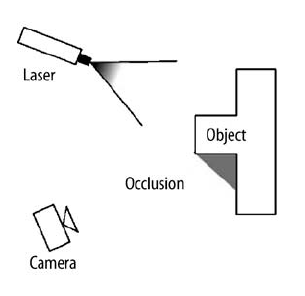
\includegraphics[width=.6\textwidth]{./images/tech/occlusion1.png}
    \subcaption{Laser occlusion}
    \label{fig:occlusions_laser}
  \end{minipage}%
  \begin{minipage}[c]{.50\textwidth}
  	\centering
    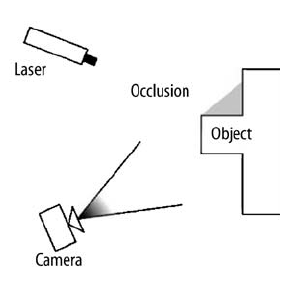
\includegraphics[width=.6\textwidth]{./images/tech/occlusion2.png}
    \subcaption{Camera occlusion}
    \label{fig:occlusions_camera}
  \end{minipage}
  \caption{Examples of different types of occlusions}
  \label{fig:occlusions}
\end{figure}

Another issue due by laser and camera relative positions, is the resolution of the camera. In 2D computer vision, the camera resolution is given by the pixel, according with the relation $resolution = \frac{Field \: of \: view}{sensor \: size}$. This is true only if the entire scene is focusable. In \acs{SOL} systems the angle between camera and laser plane prevents the focus of the entire field of view, that depends on the distance from the lens. We can distinguish three different resolutions described below. Typically, this variance in camera resolution is called \textit{trapezoidal camera resolution}. \\

\noindent
The \textit{depth resolution} is the minimum variation in the target depth appreciable by the camera. It strongly depends on the target distance from the lens and, in particular, on the angle between the projector and the camera. The greater the angle is, the greater is the variation observed in the image plane, caused by the same variation in the 3D space (in metric units). Furthermore it depends also on laser stripe thickness. Many sub-pixel approximation algorithms was developed to reduce the weight of this last factor, and some of this algorithms will be discussed later. \\

\noindent
The \textit{resolution along the laser line} is the ratio between the length of the laser line observed in the camera and the corresponding length in millimeters. As the depth resolution and because of the perspective distortion, this last resolution depends by the object distance from the camera, and it is greater close to the lens. \\

\noindent
The last is the \textit{step between consecutive frames}.
%The last is the \textit{resolution on the motion direction}.
It is present in systems that take many frames of the same object in different positions, using the same laser-camera pair. This ``resolution'' is related to the camera frame-rate and the system motion speed. \\

\noindent
The differences between them will be clearer in the Chapter \ref{ch::model}, where a complete geometric laser-camera triangulation systems model will be presented. However, we can get an idea of these differences by looking at the Figure \ref{fig:tech:resolutions}: the \textit{depth of field} is defined by the extent of the details of the focus areas. \textit{Resolution along the laser line} is given by the details appreciable by the laser itself. Finally, the tape speed and the number of captured images of the same object, define the \textit{capture step}.
  \begin{figure}[t!]
    \centering
    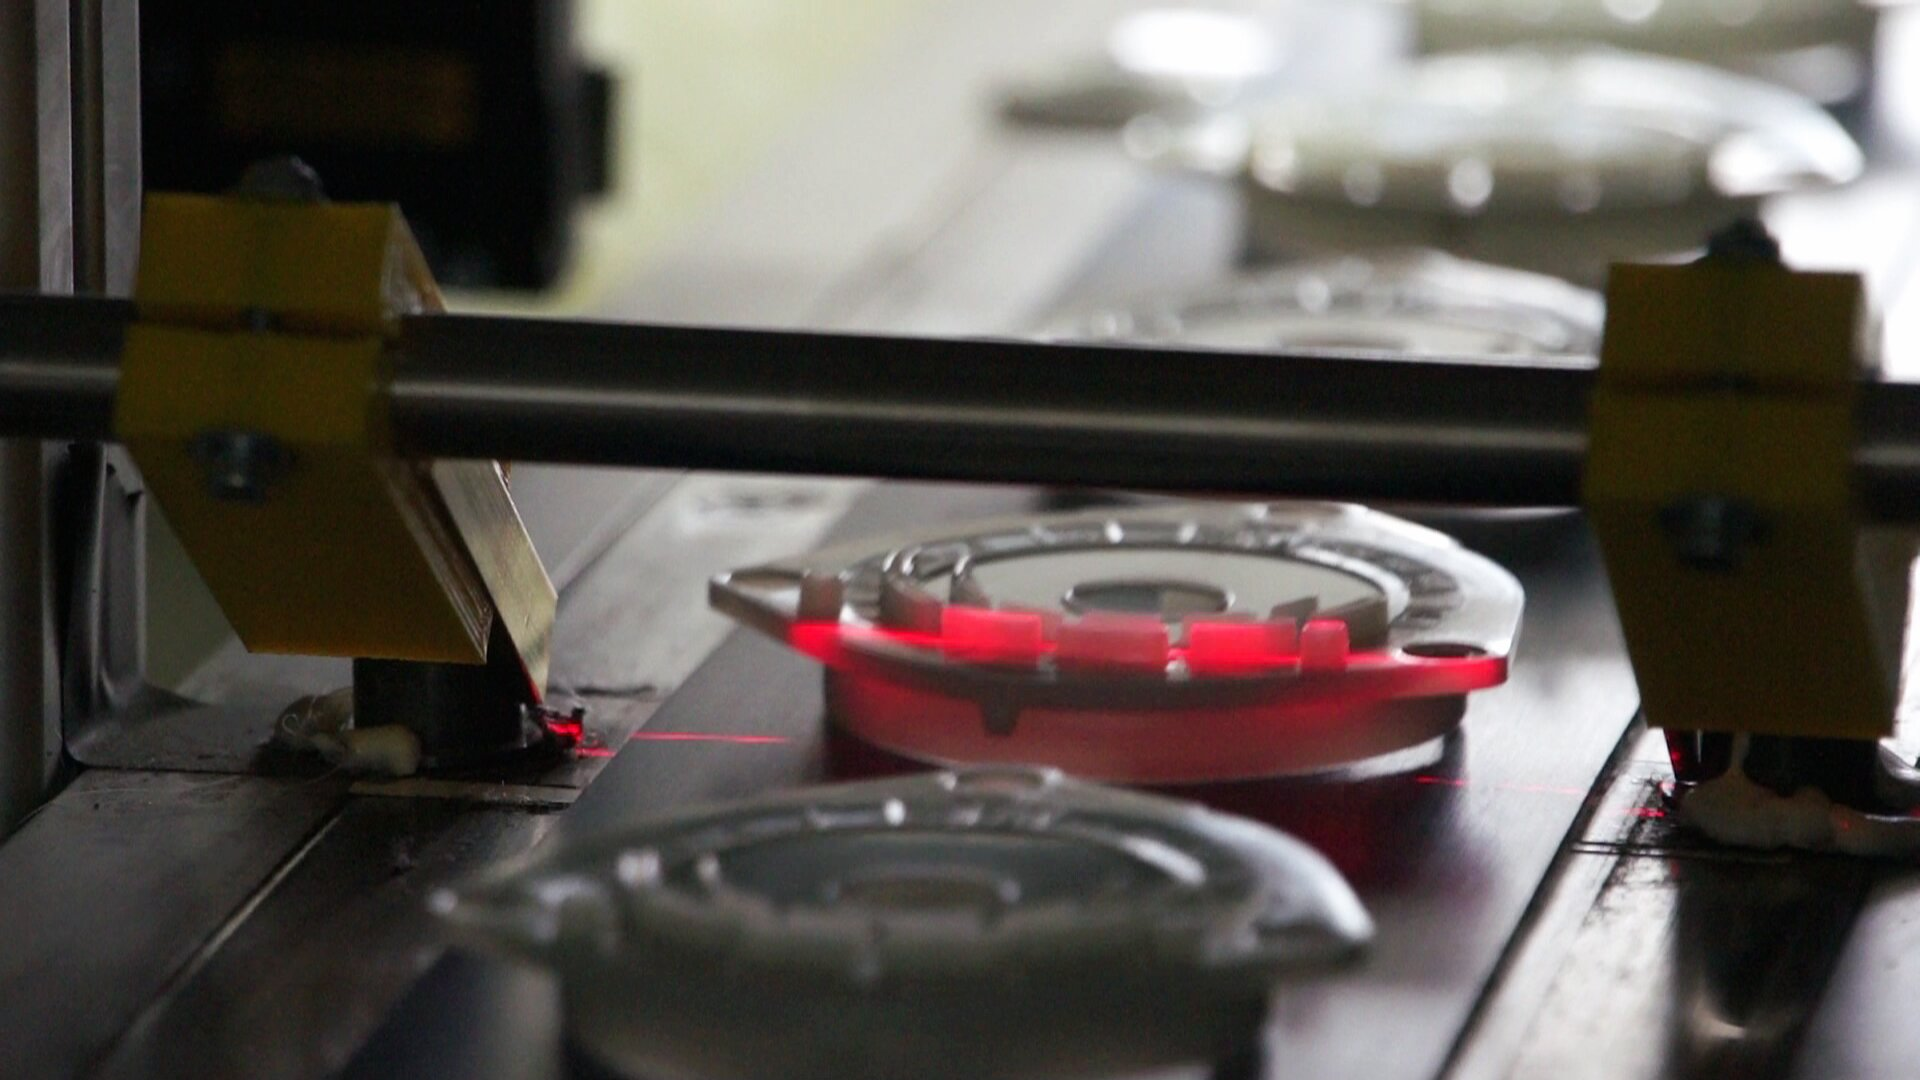
\includegraphics[width=0.8\textwidth]{./images/tech/resolutions.JPG}
    \caption{Representation of the different resolutions of a laser triangular system (property of \url{www.stemmer-imaging.co.uk}).}
    \label{fig:tech:resolutions}
  \end{figure}


% Siti di riferimento:
% http://www.vision-systems.com/articles/print/volume-20/issue-6/features/understanding-laser-based-3d-triangulation-methods.html
% http://www.aqsense.com/docs/docu_3dexpress/limits3D.html
% http://www.aqsense.com/docs/theory3D.pdf
% http://pages.stemmer-imaging.de/techforum-download/pdf/Aqsense_Understanding-and-solving-challenges-in-3D-laser-triangulation-systems_EN.pdf
% http://www.imaginasrl.it/scanner-laser.html


% Pinhole camera
  \section{Pinhole camera}
\label{sec:pinhole_camera}
Pinhole camera is the simplest camera model, where light passes through a tiny hole (from which the name \textit{pinhole camera}) of a box: an inverted image of the scene is projected on the opposite side of the box itself. This effect, known as \textit{camera obscura effect}, was studied since 500 BC (the first writings are back to the chinese Mozi) and it is the underlying principle of the $19^{th}$ century cameras. An example of the geometry of this camera is shown in Figure \ref{fig::pinhole}: as it can be seen, for each 3D point there is only one ray of light that passes through the pinhole. This is an ideal condition which allows to neglect distortions, such as blurring. Furthermore it is free of lenses, a condition that accords you to neglect distortions such as vignetting or radial and tangential distortions.
\begin{figure}[t!]
  \centering
  \begin{minipage}[c]{.48\textwidth}
  	\centering
    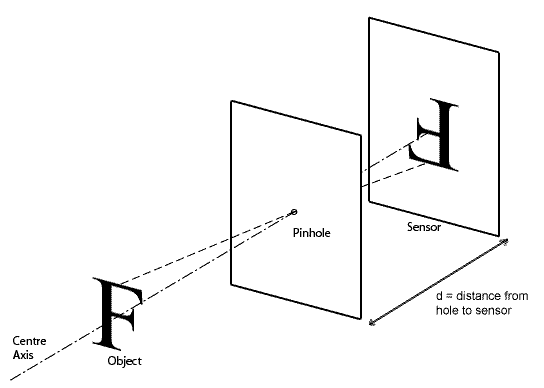
\includegraphics[width=\textwidth]{./images/tech/pinhole.png}
    \caption{The geometry of a \\ pinhole camera}
    \label{fig::pinhole}
  \end{minipage}
  \hfill
  \begin{minipage}[c]{.48\textwidth}
  	\centering
    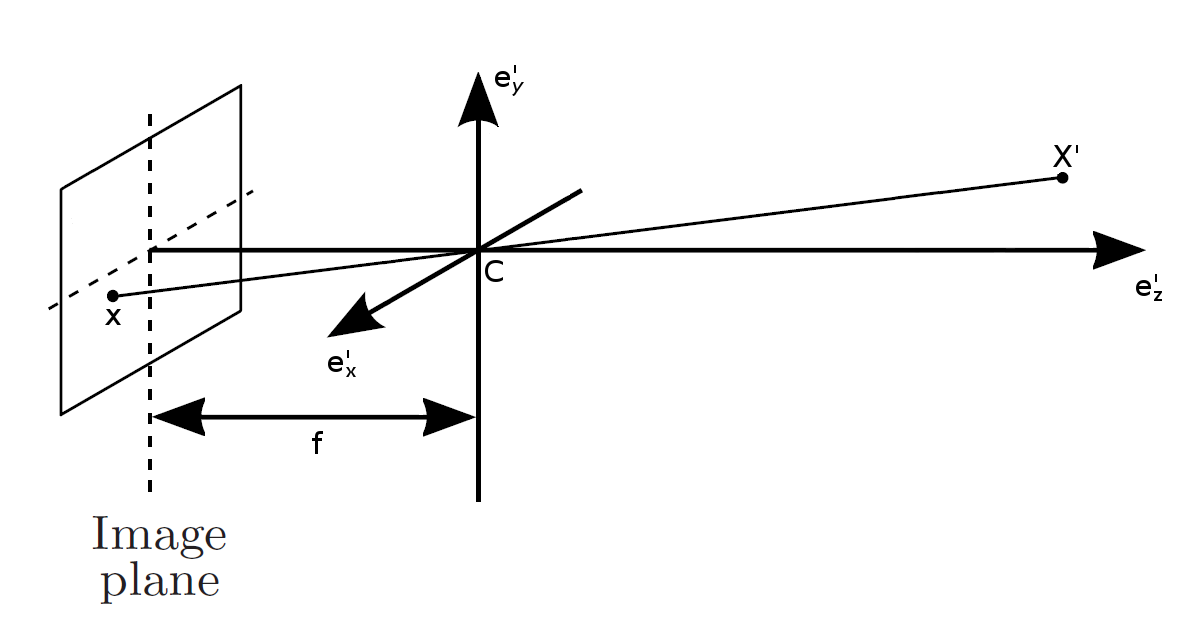
\includegraphics[width=\textwidth]{./images/tech/image_plane.png}
    \caption{Mathematical model}
    \label{fig:math_model}
  \end{minipage}
  %\caption{Examples of different types of occlusions}
  %\label{fig:occlusions}
\end{figure}

Thanks to these simplifications, the mathematical model that describes the relations between the 3D world points and their projections in the image, is very simple. Let's look at the Figure \ref{fig:math_model}. 
% Let us define the \textit{camera coordinate system} $\left(e_x', e_y', e_z' \right)$: the origin $c = \left(0,0,0 \right)$ will represent the so called camera center (i.e. the pinhole).
% We form the line between $X = \left( X_1^w, X_2^w, X_3^w \right)$ and $c$ and intersect it with the plane $z = k$ called \textit{image plane}, to generate a projection $x = (x_1, x_2, k)$ of a scene point $X$. We will refer to $e_Z$ as the \textit{viewing direction}.
% Note that if $k > 0$, the image plane is placed in front of the camera center and the image will not appear upside down. In this case we talk about \textit{virtual image}, but in real models we put $k < 0$. \\
% Since $Xc$ is a direction vector of the viewing ray we can parametrize it by the expression
%  \begin{equation*}
%    c + s(X - c) = sX \qquad s \in \mathds{R}
%  \end{equation*}
% where $sX_3^w = k$ (intersection with the plane $z = k$). Note that this model does not take into account the scene projection from the image plane to the sensor plane. \\
Let $\left(e_x', e_y', e_z' \right)$ be the \textit{camera coordinate system}, centered in $C = \left(0,0,0 \right)$, and let $C$ be the camera center (i.e. the pinhole). Then, let us define the \textit{image plane} as the 2D plane in the world in which the sensor lies. The point 2D $x = (x_1, x_2)$ in the image plane, is related to the 3D world point $X' = (X'_1, X'_2, X'_3)$ through a linear pathway for point $C$. We can parametrize this transformation with the expression:
  \begin{equation}
    \begin{pmatrix} x_1 \\ x_2 \end{pmatrix} = - \frac{f}{X'_3} \begin{pmatrix} X'_1 \\ X'_2 \end{pmatrix}
    \label{eq:image-plane}
  \end{equation}
where $f$ is the \textit{focal length} (the distance from the pinhole to which the rays are focused) of the ideal camera. This is a very simple model, but a point in the image plane does not correspond to a unique point in the world as there are three unknowns on the right hand side. Thanks to the collinearity condition from the points $X'$, $x$ and $C$, the \acs{DLT} (Direct Linear Transformation, an algorithm used to determine a set of variables from a set of similarity relations) is used: it is simple to solve this intersection and to determine this last projection. \\

However, this case is unrealistically simple, because the object and image plane are parallel. In real applications, the point $X$ can lie on a plane that have an arbitrary position and rotation, with respect to the image plane. Let us put this new plane into a \textit{global coordinate reference system} $\left( e_x, e_y, e_z \right)$; all points in the 3D world and all the camera movements will be related to this system.
% In Figure \ref{fig:math_model} we can see how point $X$ is projected in the image plane, but a questions arise: how we can locate $X$ in the world and where image plane is located respecting to the world? To answer to these questions we have to introduce a new \textit{global coordinate reference system} $\left( e_x, e_y, e_z \right)$; all points in the 3D world and all the camera movements will be related to this system.
In this way the projection of the point $X$ in the camera reference system $\left( e_x', e_y', e_z' \right)$ is a simple rotation and translation, that in \textit{homogeneous coordinates} is:
  \begin{equation}
    \label{eq:extrinsic}
    \begin{pmatrix}
      X'_1 \\ X'_2 \\ X'_3
    \end{pmatrix}
    =
    \begin{bmatrix}
      R & t
    \end{bmatrix}
    \begin{pmatrix}
      X_1 \\ X_2 \\ X_3 \\ 1
    \end{pmatrix}
    =
    H
    \begin{pmatrix}
      X_1 \\ X_2 \\ X_3 \\ 1
    \end{pmatrix}
  \end{equation}
where $R$ is a $3 \times 3$ rotation matrix and $t$ a $3 \times 1$ translation vector, and they are referred to as \textit{extrinsic parameters}, while the matrix $H$ is called \textit{homography matrix}. This is the first projection shown in Figure \ref{fig:perspective_projection}.
\begin{figure}[t!]
  \centering
  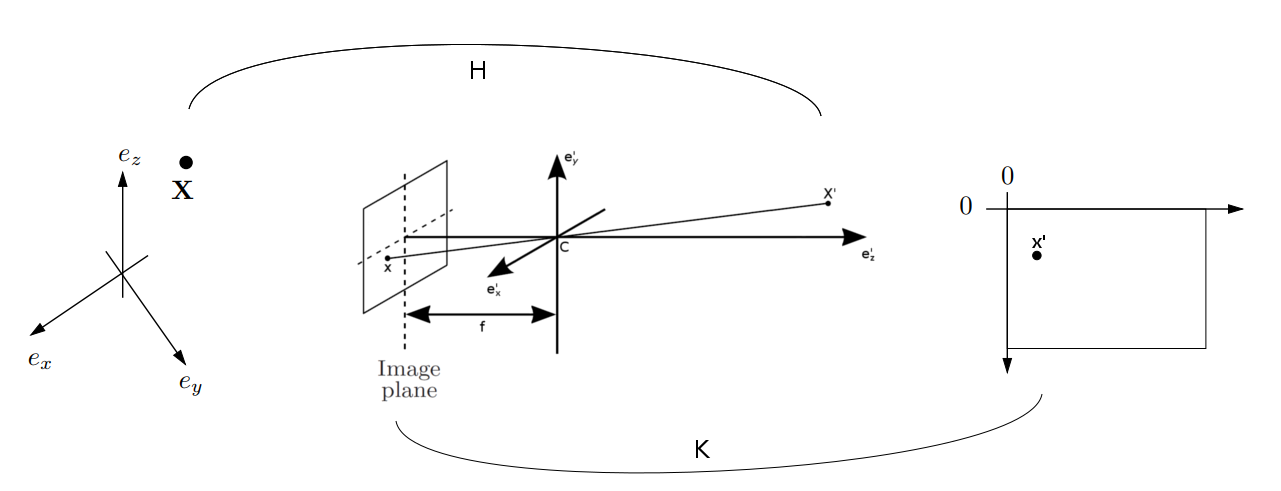
\includegraphics[width=\textwidth]{./images/tech/perspective_projection.PNG}
  \caption{Projection chain from the point $X$ in the world reference system, to $x'$ in the sensor reference system.}
  \label{fig:perspective_projection}
\end{figure} \\

The Equation \ref{eq:image-plane} shown us that the image plane is embedded in $\mathds{R}^3$, so we need to project the point $x'$ in the $\mathds{N}^2$ sensor coordinate system (in pixel unit). This is possible using a $3 \times 3$ matrix $K$ of the \textit{intrinsic parameters}
  \begin{equation*}
    \label{eq:intrinsic_matrix}
    K =
    \begin{pmatrix}
      \gamma_1	& s			& c_x \\
      0			& \gamma_2	& c_y \\
      0			& 0				& 1
    \end{pmatrix}
  \end{equation*}
where $\left( c_x, c_y \right)$ are the coordinates of the point $C$ in the sensor reference system. The pair $\left( \gamma_1, \gamma_2 \right)$ are scale factors that translate the image plane unit ($mm$) into sensor unit ($pixel$). Finally, $s$ is called skew factors, and it forces sensor rows and columns to be perpendicular. These are properties of the used camera and are related to non-ideality of camera construction. The projection (the second in Figure \ref{fig:perspective_projection}) is performed as follow:
  \begin{equation}
    \label{eq:intrinsic}
    \begin{pmatrix}
      x'_1 \\ x'_2 \\ 1
    \end{pmatrix}
    = K 
    \begin{pmatrix}
      x_1 \\ x_2 \\ 1
    \end{pmatrix}
  \end{equation} \\

The chain of all these projections, shown in Figure \ref{fig:perspective_projection}, is called \textit{perspective projection}. A common way to indicate Equations \ref{eq:extrinsic} and \ref{eq:intrinsic} in a single formula through the \textit{homogeneous coordinates} is
  \begin{equation}
    \label{eq:perspective_projection}
    \lambda
    \begin{pmatrix}
      x_1 \\ x_2 \\ 1
    \end{pmatrix}
    = KH
    \begin{pmatrix}
      X_1 \\ X_2 \\ X_3 \\ 1
    \end{pmatrix}
  \end{equation}
where the parameter $\lambda$ takes into account the projection in Equation \ref{eq:image-plane}.

%--------------------------------------------------%
\subsection{Lenses}
\label{subsec:lenses}
As mentioned above, Equation \ref{eq:perspective_projection} does not consider many non-ideality that affect the quality of images acquisitions. 

In Section \ref{sec:pinhole_camera} we introduced the fact that, ideally, only one ray per point passes through the pinhole. If on the one hand this guarantees focus, on the other the impression of the scene in the sensor requires too much time. The increasing of the size of the pinhole allows the passage of light, reducing sensor exposure time. However, in this case the projection of the point on the sensor is the result of the mixing of many light rays, condition that reduces the image sharpness until becomes a continuous smear. Lenses are used to solve this problem.

The role of the lenses is the same as the pinhole: in fact, it allows the passage of light. Their advantage compared to the pinhole is the ability to converge many light rays on a specific point, allowing much more light, and reducing film exposure times. Lens models can be quite complex, so a common practice is considered: the \textit{thin lens approximation}. A thin lens is a lens with a negligible thickness compared to the radii of curvature of its surface. In this way Equation \ref{eq:perspective_projection} remains the same. Despite this, the use of lenses introduces some other issues. \\

The amount of light that impresses the sensors is proportional to the lens diameter. The bigger the diameter is, the more light enters in the camera, but we have to consider also the \textit{magnification}. Magnification is the process of enlarging (factor greater than one) or decreasing (factor less than one, this situation is also called ``minification'') appearance of something. In this case magnification refers to the ability to see more details of the world in a single image. That said, the brightness of the image depends inversely on magnification. A simple way to indicate \textit{aperture} of a lens (the opening through which light travels), is using the \textit{f-number} $K$, defined as
  \begin{equation}
    K = \frac{f}{d}
    \label{eq:fnumber}
  \end{equation}
where $f$ is the lens focal length and $d$ the aperture diameter. As we can see in Equation \ref{eq:fnumber}, $K$ decreasing at increasing of $d$. Thanks to $K$, it is possible to compare lenses, considering image luminosity, focal length and magnification. Note that this is a simple rule with no effects on the Equation \ref{eq:perspective_projection}. \\
  
Another problem is the focus of the lens. While a pinhole camera is permanently on-focus (ideal condition), this is not always valid for a lens. In reality a lens is on focus only at a specific distance: this means that only the point at that distance will be perfectly sharp. All the other points that are out-of-focus are projected on film as circles, called \textit{circles of confusion}. The blur spot shape is due by the aperture shape (that typical is a circle from which the name) and its size increases with the distance from the focus plane. Differently from chemical film, digital sensor are made as a matrix of photosensitive elements (pixels) that convert light in electrical signals; this means that sensors resolution is not infinite. If the circle of confusion is smaller than pixels sizes, we can consider that point on focus. The space range, around the focus plane in which the scene looks reasonably sharp, is called \textit{depth of field} (\acs{DOF}). An example of these effects, common in literature, is shown in Figure \ref{fig:dof}.
%  \begin{wrapfigure}{L}{0.5\textwidth}
%    \centering
%    \includegraphics[width=0.5\textwidth]{./images/dof_txt.jpg}
%    \caption{Example of a very shallow \acs{DOF}.}
%    \label{fig:dof}
%  \end{wrapfigure} \\
  \begin{figure}[t!]
    \centering
    \begin{minipage}[c]{.48\textwidth}
      \centering
 \includegraphics[width=\textwidth]{./images/tech/dof_txt.jpg}
      \caption{Example of a very shallow \acs{DOF}.}
      \label{fig:dof}
    \end{minipage}
    \hfill
    \begin{minipage}[c]{.48\textwidth}
      \centering
 
\includegraphics[width=0.74\textwidth]{./images/tech/airydisk.jpg}
      \caption{Example of an \textit{airy disk}.\\ ~}
      \label{fig:airy-disk}
    \end{minipage}
  \end{figure} \\

The second big advantage of lenses against the pinhole, is the reduction of the diffraction. Diffraction is an effect generated by the interferences of light waves, when the light finds an obstacle or a hole, similar to the size of its wavelength. As the divergent rays now travel to different distances, some of them move out of phase and begin to interfere with each other, adding in some places and partially or completely canceling out in others. This effect, well known in many fields of interest, from electromagnetic to sound, in photography is known as \textit{airy disk} (by his discoverer, George Airy) and it is shown in Figure \ref{fig:airy-disk}. As for \acs{DOF}, even diffraction is negligible if it is smaller than the size of pixels. Diffraction could be present also in the \acs{DOF} of the camera, and depends only by the $f$-number, not by focal length. Lenses reduce this noise on the image, setting their aperture up appropriately. \\

Regardless of the lens model chosen (i.e. thin or thick lenses), their use introduces distortions due to the nature of the lens itself. In geometric optics, a distortion is a deviation from rectilinear projection, caused by small blemishes in the lenses and their alignment. The main optical aberration are two: \textit{radial distortion} and \textit{tangential distortion}. \\
Almost all of the deformation is radial in nature, this is the reason why distortion are more apparent from the center toward the edges of the image. This particular type of distortion is able to change the direction of straight lines, and it is evident during 3D calibration phases, when straight reference objects are seen from the camera as curve. Furthermore, it is often due to the need to expand the field of vision using a camera with short focal distance. Some example of its effects can be seen in Figure \ref{fig:teo-distorsions}. \\
Vice versa, tangential distortion is typically negligible than radial one, then it is ignored in most mathematical models.
  \begin{figure}[h!]
    \centering
 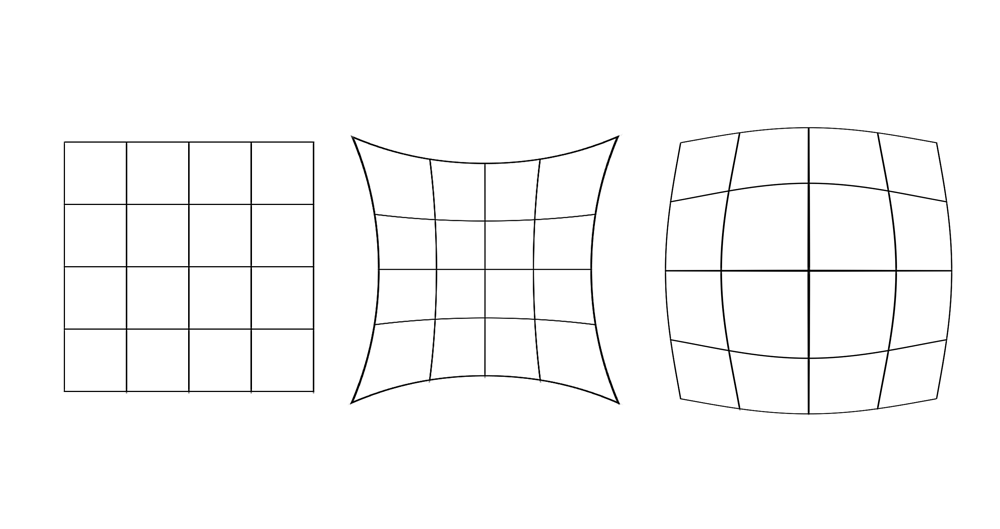
\includegraphics[width=0.9\textwidth]{./images/tech/distorsions.png}
    \caption{Example of radial distortions: on the left distortions free image is shown; in center a \textit{pincushion} aberration; on the right a \textit{barrel} aberration.}
    \label{fig:teo-distorsions}
  \end{figure}

%--------------------------------------------------%
\subsection{Scheimpflug principle}
In the previous subsection we talked about \acs{DOF} and the problem to maintain focus on the whole scene. Furthermore, we dealt with the Figure \ref{fig:dof} to show the result. Anyway, in the figure we can see that the subject lies on a plane not parallel with the sensor plane. Typical cameras and lenses are designed so that sensor plane, lens plane and subject plane are parallel to each other. This makes the focus of the camera very simple but, as said in Subsection \ref{subsec:lenses} talking about the rectilinear projection, the effective focal length depends by the position of the target with respect to the sensor itself. \\

Since the early $20^{th}$ century, the study of rotating the lens with respect to the sensor, and its effects on image acquisition, has been a widespread practice. In $1901$, Carpenter (one of the fathers of cinema) patented the first prototype of the so called ``view camera'' \cite{pat:carpentier}. From these studies, the Captain T. Scheimpflug patented \cite{pat:scheimpflug} in 1904. With his patent, Scheimpflug was the first to formulate the mathematical problem. The \textit{Scheimpflug principle} is a geometric rule that describes the relations between the sensor plane, then lens plane and the plane of focus when the lens plane is not parallel to the image plane. To achieve this situation, some cameras, such as view cameras, allow to tilt either the lens and the film, relative to the other. \\
  \begin{figure}[b!]
    \centering
    \begin{minipage}[c]{0.49\textwidth}
      \centering
      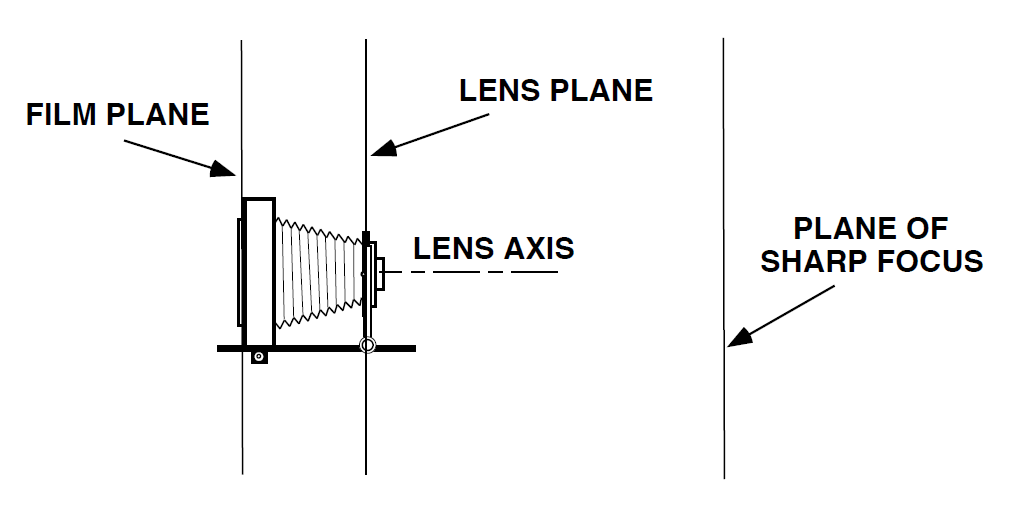
\includegraphics[width=\textwidth]{./images/tech/sch_par.png}
    \end{minipage}
    \hfill\
    \begin{minipage}[c]{0.49\textwidth}
      \centering
      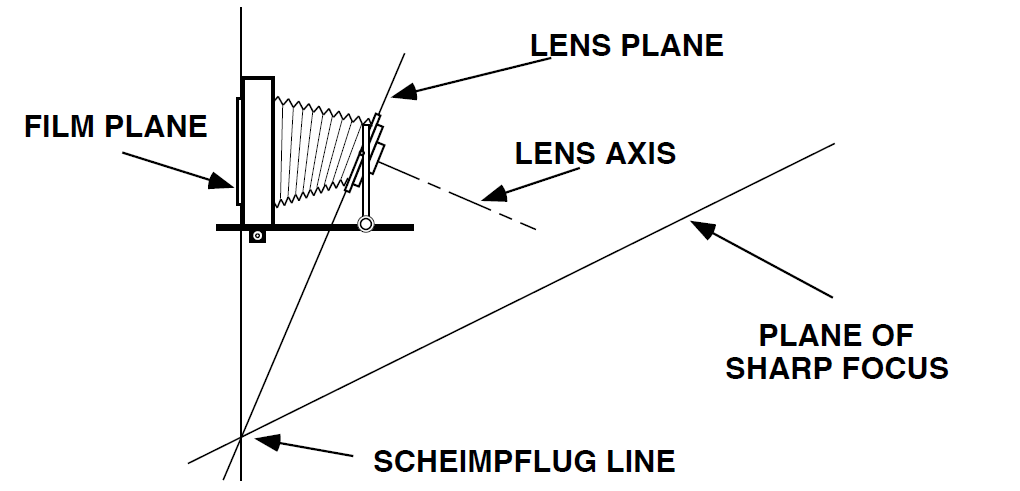
\includegraphics[width=\textwidth]{./images/tech/sch_tilt.png}
    \end{minipage}
    \caption{(On the left) For standard cameras, the sensor, lens and focus planes are parallel to one another. (On the right) For a view camera, tilting lens causes the plane of sharp focus to tilt as well.}
    \label{fig:scheimpflug}
  \end{figure}

This principle asserts that when the lens is tilted, lens plane, image plane and the plane of focus all intersects in a line, called \textit{Scheimpflug line}, as illustrated in Figure \ref{fig:scheimpflug}. In this way, a subject that is not parallel to the sensor can be completely in focus. Nevertheless, this first relation does not give any information about how to tilt the lens to achieve the intended position for the plane of focus. This information arises from the laws of optics, thanks to the \textit{hinge rule}, similar to Scheimpflug one. The required amount of lens tilt is given by the expression:
  \begin{equation*}
    \alpha = \arcsin \left( \frac{f}{J} \right)
  \end{equation*}
where $f$ is the focal length of the lens, and $J$ is the distance from the lens and the \textit{hinge line}. The hinge line is the intersection between a plane parallel with the sensor and passing through the lens one, and the plane of focus. \\
From this principle we can also determine the \acs{DOF} of the camera. It can be demonstrated that the limits of the \acs{DOF} are also planes, that passes through the hinge line, and symmetrical compared to the plane of focus. To be precise, these planes lies at a distance $J$ from the plane of focus, distance measured at the \textit{hyperfocal distance} $H$ from the hinge line \cite{book:ftvc}. The scenario is illustrated in Figure \ref{fig:sch_dof}.
  \begin{figure}[h!]
    \centering
    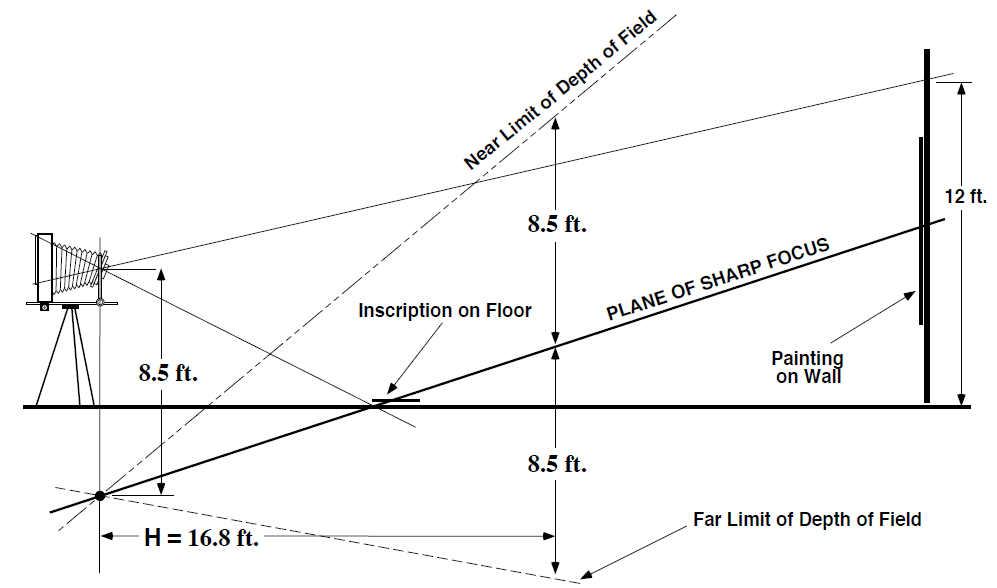
\includegraphics[width=0.8\textwidth]{./images/tech/sch_dof.png}
    \caption{Depth of field in view cameras, with tilted lenses.}
    \label{fig:sch_dof}
  \end{figure}

%--------------------------------------------------%
\subsection{Overview on digital cameras}
\label{subsec:overview-cameras}
To complete the introduction on digital camera we think that it could be useful to linger over some practical aspects, in particular about what concerns manufacturing of the sensor and image acquisitions. \\

In Subsection \ref{subsec:lenses} we introduced the quantization effect due by pixels. If it relaxes the problem of the lens focus, on the other hand it introduces noise in light to image conversion. We briefly analyse the two most popular sensor types on the market: \acs{CMOS} and \acs{CCD} (Charge-Coupled Device).

In \acs{CMOS} sensors, each element has its own signal amplifier: this allows to improve the camera frame rate and to isolate regions of interests via hardware. On the contrary, pixels haven't the same sizes neither the same doping, which reduces the quality of the sensor itself. The latest CMOS sensors on the market are good enough to be used in computer vision, achieving excellent results.

\acs{CCD} are high-scale integration sensors that use only one signal amplifier, ensuring the same amplification constant for each element. However, this requires that sensor rows are converted one by one, by lowering the camera frame rate. Furthermore these sensors give a very small, but non-zero response to a zero input and they saturate for very bright stimuli. In spite of that, they are much less noisy than the CMOS.

These differences are very delicate, specially considering the fields of application of the camera. For example, in laser triangulation systems, the acquired images are dark to highlight the laser light. In situation like this, when the brightness of the image is very low\footnote{In this case we consider source of light with brightness near to the base noise level of the sensor.}, signals amplification offsets are meaningful. The mono-pixel amplifiers in \acs{CMOS} are more noisy and generate less uniform values than \acs{CCD}, resulting in a more homogeneous output. This source of noise is known as \textit{thermal noise}. High quality systems provide different solutions to reduce this effect as much as possible. In Figure \ref{fig:thermal-noise} an example of the noise is shown.
  \begin{figure}[h!]
    \centering
    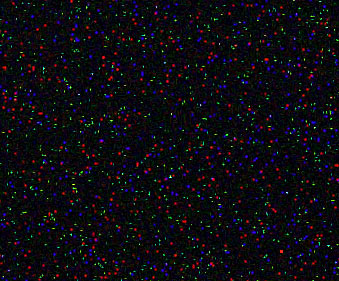
\includegraphics[width=0.5\textwidth]{./images/tech/dark-example.jpg}
    \caption{Example of uncontrolled dark noise in astronomical photography.}
    \label{fig:thermal-noise}
  \end{figure} \\

Another problem due to sensor quantization, is colours acquisition. Each pixel is able to acquire only light signals, resulting in grey scale acquisitions. For this reason sensors needed filters to encode colours. The most widespread is \textit{Bayer's color filter array} (Bayer's \acs{CFA}). A \acs{CFA} is an array in which passband filters are placed, according to a known pattern. In this way each pixel is able to encode only a specific colour. Many algorithms are used to reconstruct the scene; they interpolate signals collected by near pixels and extract the correct colour for each pixel. To perform measures, this is a waste of pixels: the presence of the filter reduces the sensor surface useful to collect world details. For these reasons, grey scale cameras are often used.


% Active light sources
  \section{Active light sources}
% According to Scott Palmer in his book Light (2013), passive and active light were at the core of Adolphe Appia's creative vision. 'The passive or diffused light refers to the general light of the stage area usually from footlights and border lights, which were common to existing stage practices at the end of the nineteenth century and were principally concerned with the widespread illumination of the stage space. In contrast, active light refers to intense, focused light that crucially allows distinct shadows to be created.
In 3D machine vision, there are many sources of light, used by the cameras to collect the information of interest. We can group these sources into two sets: \textit{passive} and \textit{active} sources. The first set refers to reflected light (typically used in photography), that is ``the general light of the stage area [\ldots] and were principally concerned with the widespread illumination of the stage space'' \cite{palmer2013light}. The second set refers to all intense and focused lights that create distinct shadows on the scene.
% Per quanto riguarda i sistemi basati su triangolazione ...
As far as triangulation-based systems are concerned, we are only interested in active sources, in particular in \acs{LASER}. \\

A \acs{LASER} is a device that emits a coherent light beam, and originally its name was the acronym of \textit{Light Amplification by Stimulated Emission of Radiation}. It comes from the physical processes used to generate the light beam: when an incoming photon (at a specific frequency) interacts with an excited electron, the electron changes its energy level. The energy liberated when it returns to its initial state, generates a new photon, completely identical to the first one. Now, the four main parts that compose this device are:
  \begin{itemize}
    \item The \textit{active medium} is the source of optical gain.
    \item The \textit{pumping system}, that provides the energy needed to excite photons.
    \item The \textit{cavity resonator}, where the photons are reflected back and forth between the cavity's walls.
    \item The \textit{collimator}.
  \end{itemize}
As far as the last point is concerned, it is not a fundamental element from the point of view of the \acs{LASER} itself, but for its use in measuring systems. In fact, as we will describe later, the emitted light has the shape of a spot. To spread it along a line, a collimator is needed. A collimator is a particular curved lens, putted in front of the \acs{LASER}, that filters the stream of rays so that only those travelling parallel to a specified direction are allowed through. In this way, it is possible to spread the light power on a plane and to obtain a \acs{LASER} line on the target.\\

The main properties of the \acs{LASER}s are their temporal and spatial coherences. The spatial coherence allows the \acs{LASER} to be collimated: this means that the rays of light are all parallel to each other, generating the typical shape of a spot. For this reason, in \acs{SOL} systems it is common to put a \textit{collimator} in front of the \acs{LASER}, in this way the energy of the collimated spot is spread to a plane, that is a line when it hits a target object. \\
Temporal coherence, instead, allows the \acs{LASER} to emit light with a very narrow spectrum, i.e. they are monochromatic. \\
Thanks to their coherencies, the \acs{LASER}s can focus a great amount of energy on a very small areas, allowing their use in a wide range of applications. Depending on the field of application, we can find \acs{LASER}s with different wavelengths, both in visible and invisible spectrum. \\

  \begin{table}[b!]
  \begin{tabular}{|c|p{12cm}|}
  \hline
  \multicolumn{1}{|c|}{\textbf{Class}} & \multicolumn{1}{c|}{\textbf{Description}} \\
  \hline
  
  1  &
  \acs{LASER}s that belong to this class are always safe for the human health. Generally the emitted power is $P < 0.04 mW$, but in this class there are also that \acs{LASER}s that prevents the direct interaction of the operator (such as laser printers). No protection is required. \\
  \hline
  
  1M &
  This class differs from the previous one because these are dangerous \acs{LASER}s, if used in pair with optical instruments. Typically, their works in the range $\left[302.5, 4000\right] nm$. \\
  \hline
  
  2  &
  These are low-power \acs{LASER}s $\left( P < 1 mW\right)$ that emit in the visible spectrum $\left( 400, 700 \right) nm$. This type of \acs{LASER}s are not inherently safe, but the eyelid is enough to protect eyes from incidental reflections. It is important not to look them directly. \\
  \hline
  
  2M &
  Like the class 1M, \acs{LASER}s belonging to this class refer to class 2 too, but are dangerous if used in pair with optical instruments. \\
  \hline
  
  3R &
  This is the first class of \acs{LASER}s that are really dangerous for humans. Here we find \acs{LASER}s that emit in the visible spectrum $\left(302.5, 106\right) nm$. They can injure eyes even if viewed indirectly. \\
  \hline
  
  3B &
  Like the class 3R, we can find \acs{LASER}s dangerous both for eyes and skin. They emit beams with power under $500 mW$. \\
  \hline
  
  4  &
  Like the class 3B, \acs{LASER}s that belong to this class are dangerous for eyes and skin, even in diffuse radiation, and they can cause fires. Another source of danger are their very high working voltage and current. We have to be very careful when we use this class. \\
  \hline
  \end{tabular}
    
  \caption{Classes of \acs{LASER}s and their regulations} 
  \label{tab:laser-classes}
\end{table}
Nevertheless, lasers coherence can be a risk factor for the health of users. Because of their differences in wavelength, emitted power and pulse frequencies, it has been necessary to rule their use, and to group them, accordingly with their properties. \acs{CEI} grouped \acs{LASER}s in five classes, accordingly with regulations \cite{cei:76-2}, in order to define the \acs{MPE} (Maximum Permissible Exposure) for each category, i.e. the maximum exposure time in which the damage for the health is negligible. These classes are described in Table \ref{tab:laser-classes}. The choice of the correct class needed in our project is very important, in particular in industrial systems. For our tests, described later, we used \acs{LASER}s belonging to classes 1 and 2. \\

% --------------------------- %
\subsection{Peak detection}
\label{subsec:peak-detection}
An important aspect of lasers is their mathematical modelling. The accuracy of triangulation-based systems, and in general of laser-based systems, is significantly determined by the detection of the laser stripe. \\

In literature there are many models that try to describe laser stripes, but the most used is the \textit{Gaussian} shape that, accordingly with \cite{saleh2013fundamentals}, we can generalize as:
  \begin{equation}
    e^{-jkz}
    \label{eq:general-gauss-model}
  \end{equation}
where $k = \frac{2\pi}{\lambda}$ is the wavenumber with wavelength $\lambda$, and $z$ is the direction of propagation of the signal. This model is quite simple, because it approximates the spot laser with the point of maximum light intensity (peak of the Gaussian). Furthermore this model is symmetrical with respect to the center of the spot, guaranteeing the shape shown in Figure \ref{fig:laser-spot-gauss}. Like camera lenses, also lasers have to be focused. Since the beam has its minimum width at $z = 0$, this will be the best focus plane. Moving in both directions, the width of the beam grows ``out of focus''. When the width of the beam is $\sqrt{2}$ the initial width, we have reached the laser \textit{depth of focus}.
  \begin{figure}[t!]
  \centering
    \begin{minipage}[c]{.48\textwidth}
      \centering
      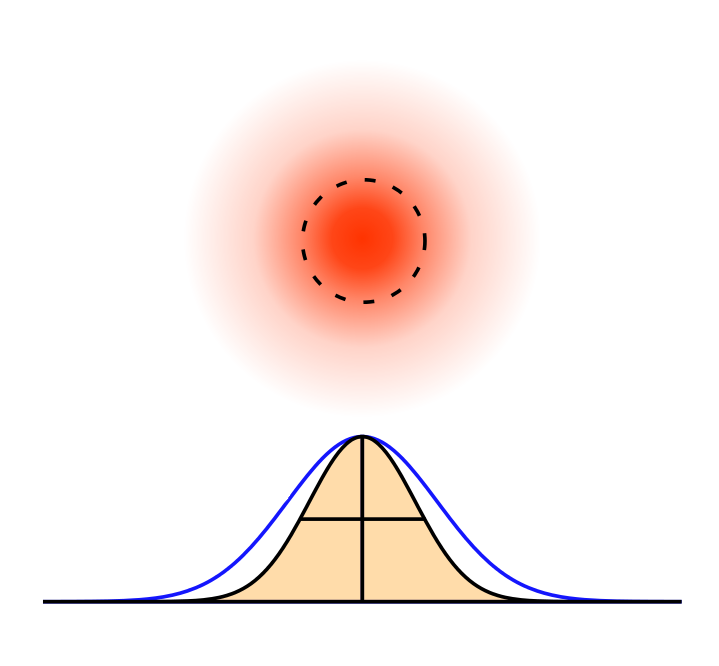
\includegraphics[width=0.8\textwidth]{./images/tech/laser-gauss.png}
      \subcaption{Gaussian model.}
      \label{fig:laser-spot-gauss}
    \end{minipage}
    \hfill
    \begin{minipage}[c]{.48\textwidth}
      \centering
      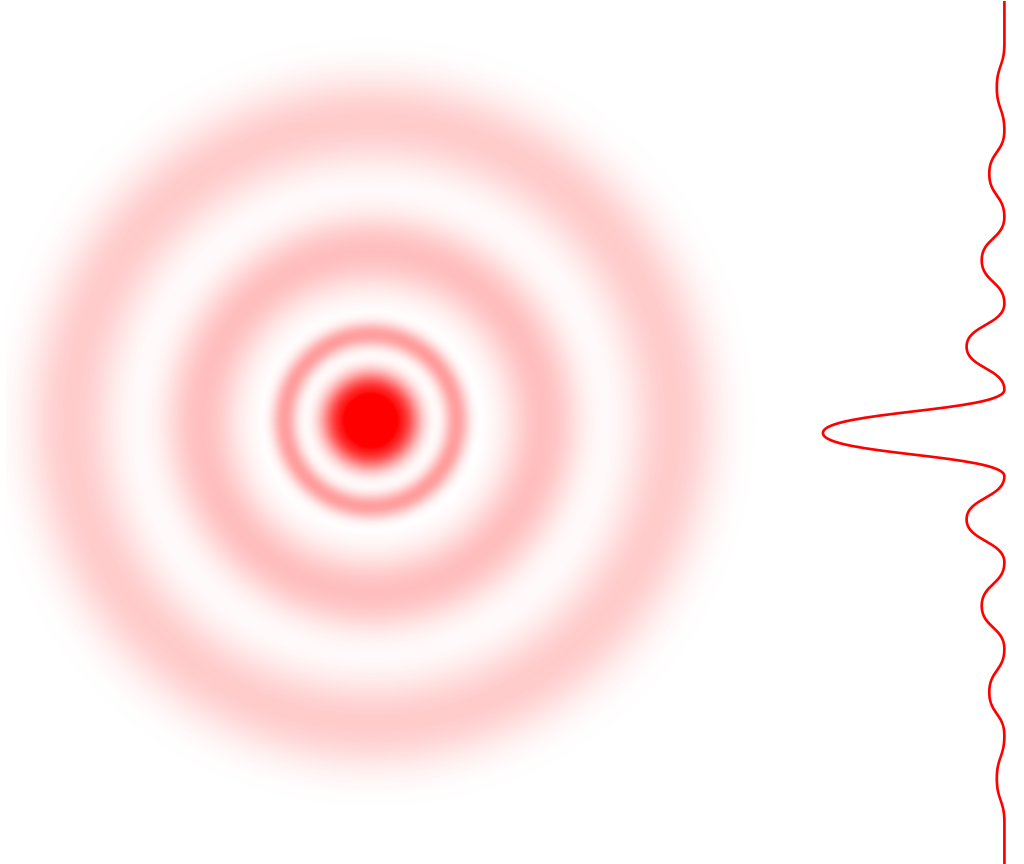
\includegraphics[angle=270, origin=c, width=0.64\textwidth]{./images/tech/laser-bessel.png}
      \subcaption{Bessel model.}
      \label{fig:laser-spot-bessel}
    \end{minipage}
    \caption{Models for lasers spots.}
    \label{fig:laser-spot-models}
  \end{figure}

Another solution, proposed in \cite{saleh2013fundamentals}, is the \textit{Bessel} laser model. As we can see in Figure \ref{fig:laser-spot-bessel}, this model is very similar to the Gaussian one: it has a global maximum and it is symmetrical with respect to its center. The interesting thing is the fact that it is diffraction free and has a bigger depth of field than the Gaussian model. \\

Before going deeper in the problem of laser extraction from an image, it is important to introduce the \textit{speckle noise}. Speckle noise is a granular noise that inherently exists in all coherent sources (lasers, radars, SAR, ...). It is generated when a coherent signal strikes a rough surface, spreading random radiation into space. Thanks to their coherence, the radiations are identical to the original signal, but some of them change their phase, interfering with each other. The interferences can be constructive or destructive, and what we see in the image plane is a dotted spot. The effects of this noise change if we vary the wavelength of the laser, the aperture of the lens and the setup of triangulation system, but the main important thing is that, accordingly with \cite{Baribeau:91},\cite{Dorsch:94} and \cite{Hausler:88}, this noise is a limit for the determination of the precise position of the spot in the image. \\

Once we have defined these models, the next step is to locate the laser position in the image. To do that, we can consider each row of the image as a Gaussian, defined by the value of the pixel belonging to that row, as shown in Figure \ref{fig:tech:laser-prof}. Thanks to shape and symmetry of the Gaussian distribution, it is common to look for the pixel of greatest light intensity, that ideally is located under the peak of the laser. Using this approach for each row of the same frame, we can obtain the results shown in Figure \ref{fig:tech:laser-example}.
%Once we have defined these models, the next step is to locate the laser position in the image. To do that, we can consider each row of the image as a Gaussian, defined by the value of the pixel belonging to that row. In Figure \ref{fig:tech:laser-prof} we shown a representation of this assumption. Thanks to shape and symmetry of the Gaussian distribution, it is common to look for the pixel of greatest light intensity, that ideally is located under the peak.
% Once we have defined these models, the next step is to locate the laser position in the image. Thanks to their shape and symmetry, it is common to look for the pixel of greatest light intensity, that ideally is located under the peak.
However, as we can see in Figure \ref{fig:gauss-discr} this is not completely correct: the discretization introduced by the physical structure of the sensor, forces the Gaussian to stay in the middle of the pixel, and in some cases (such as the one illustrated in Figure) if the peak is between two pixels, we make an error regardless of the pixel we choose. From the point of view of the accuracy of the measure, this approximations are too coarse to satisfy the typical industrial requirements. \\

  \begin{figure}[t!]
    \centering
    \begin{minipage}{\textwidth}
      \centering
      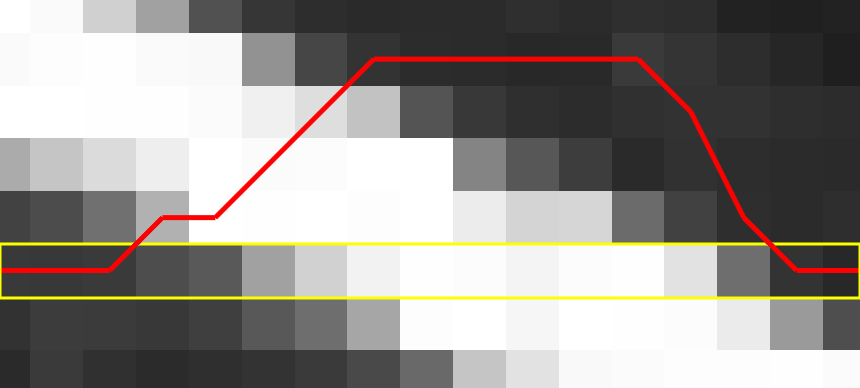
\includegraphics[width=0.8\textwidth]{./images/tech/laser_prof.png}
      \caption{Gaussian approximated distribution of the highlighted line.}
      \label{fig:tech:laser-prof}
    \end{minipage}
    \vfill
    \begin{minipage}{0.49\textwidth}
      \centering
      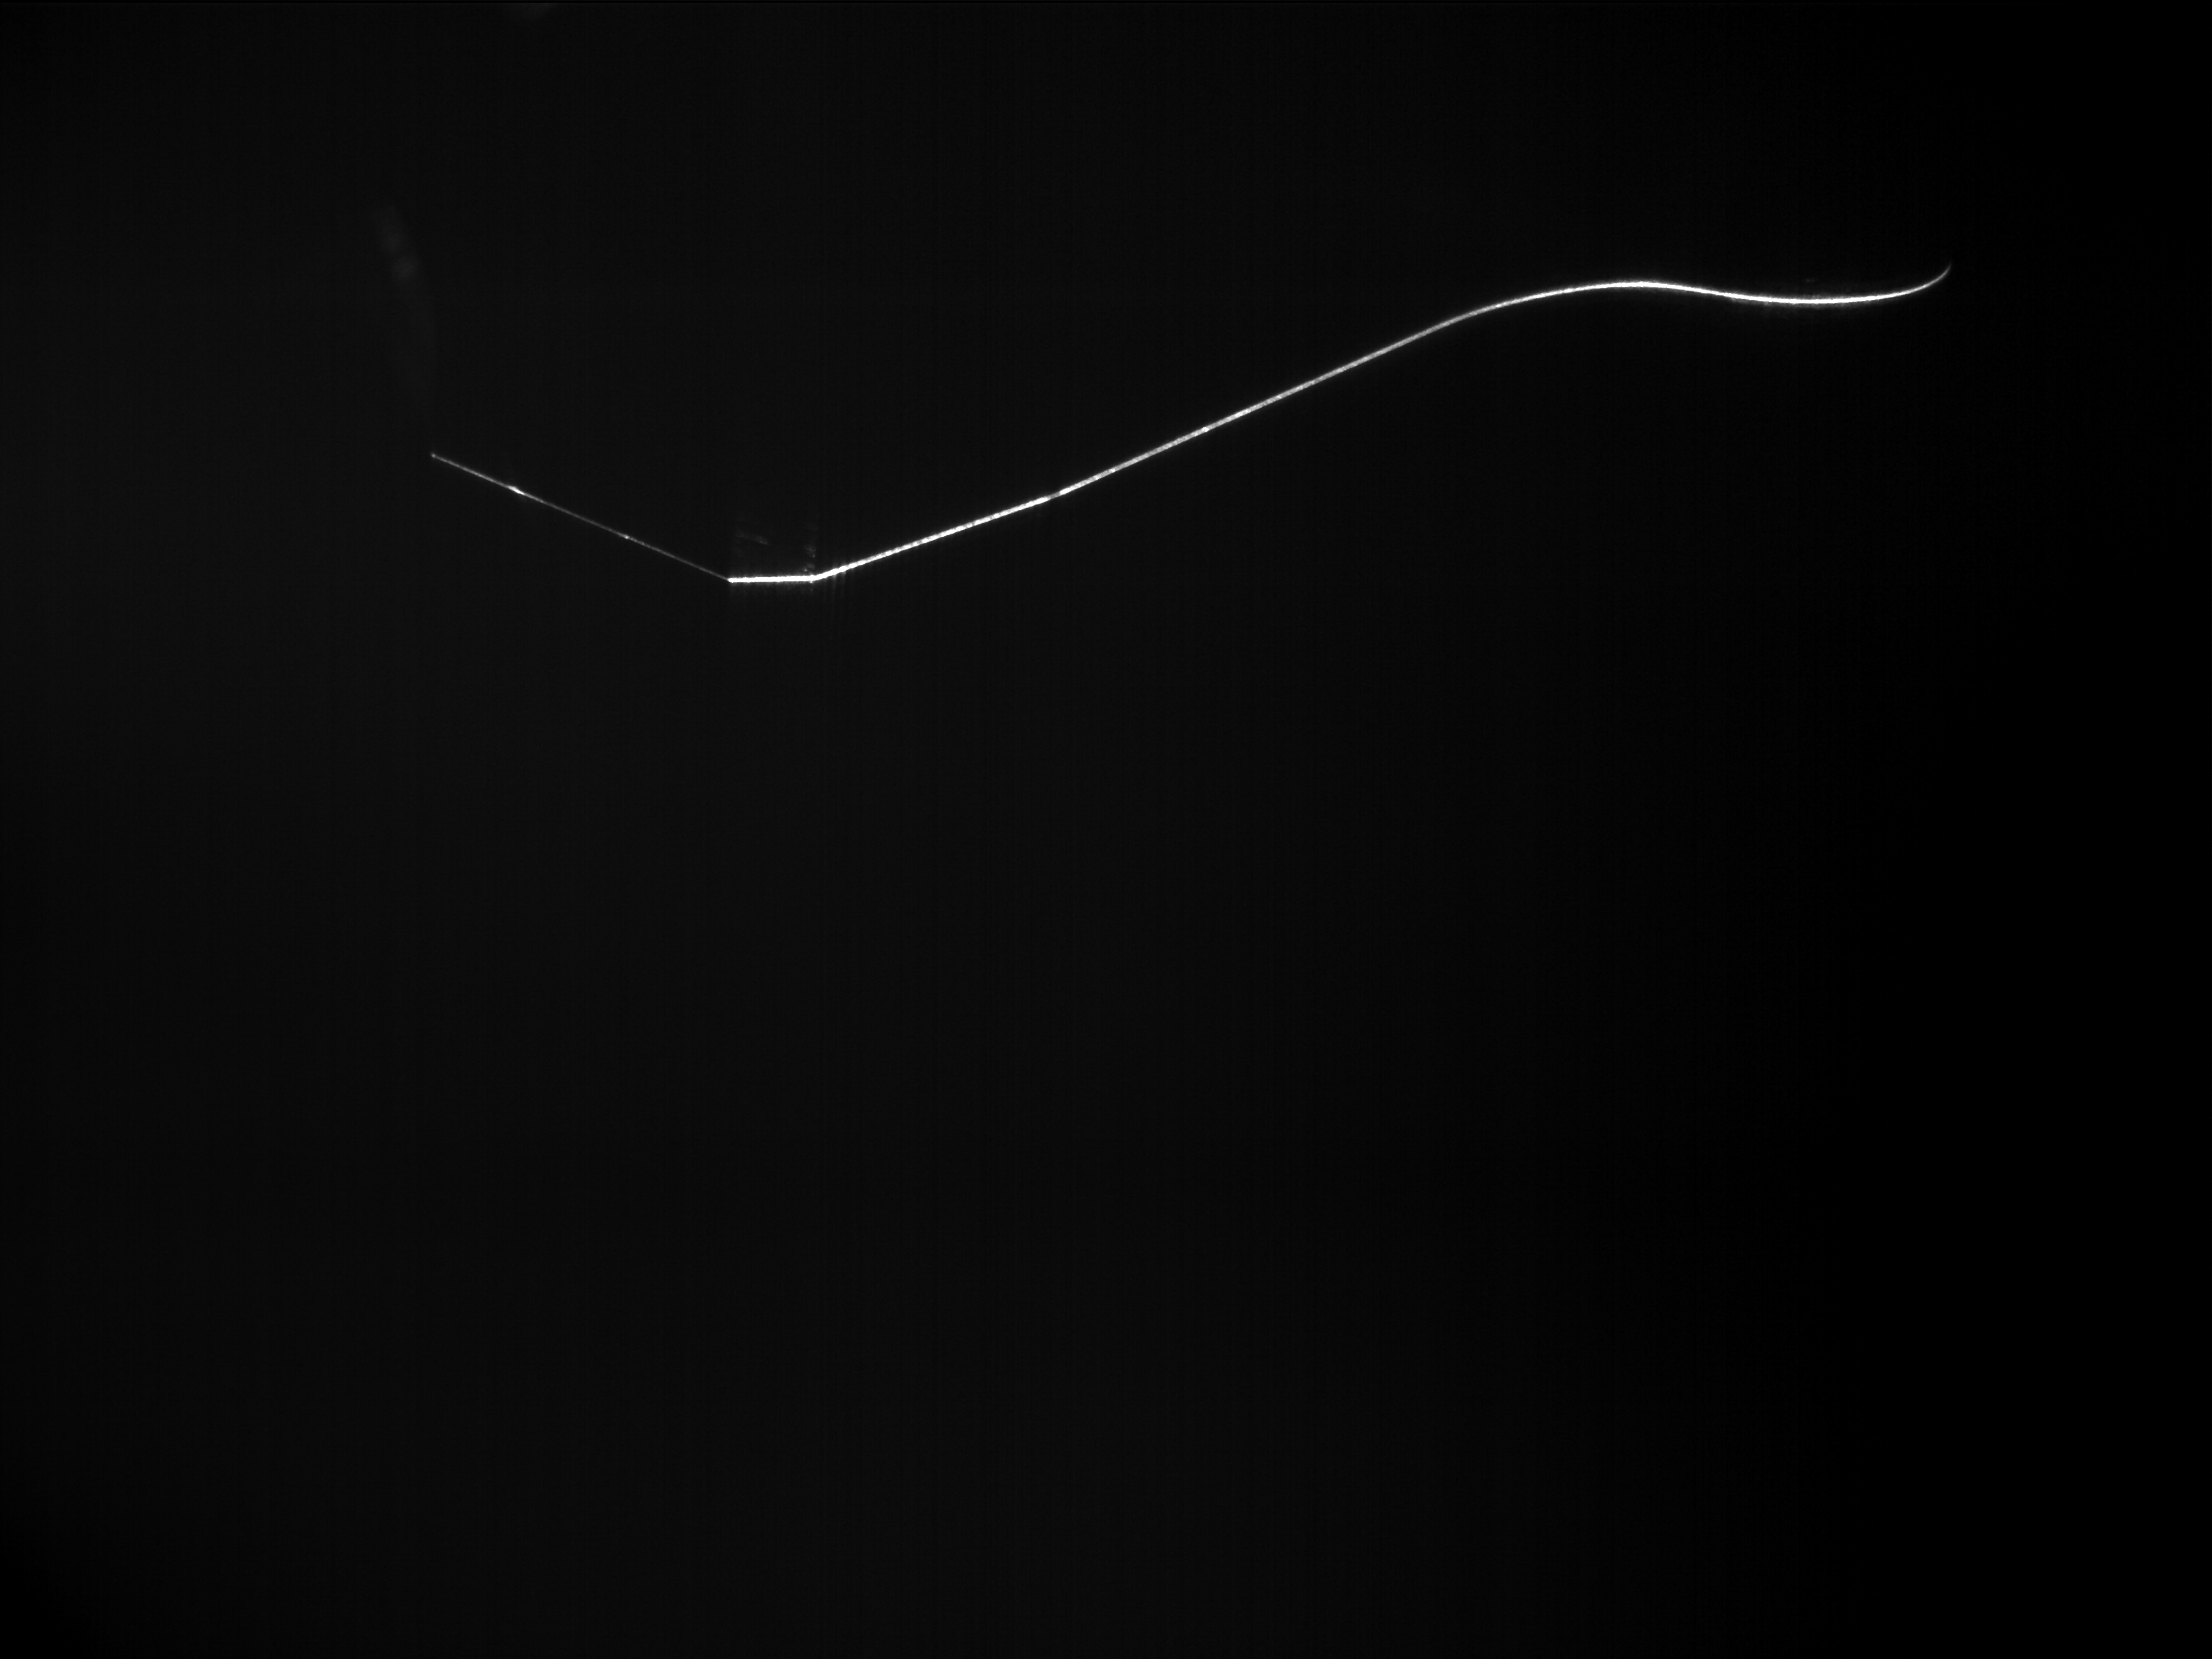
\includegraphics[width=\textwidth]{./images/tech/C0_p240_SD.png}
    \end{minipage}
    \hfill
    \begin{minipage}{0.49\textwidth}
      \centering
      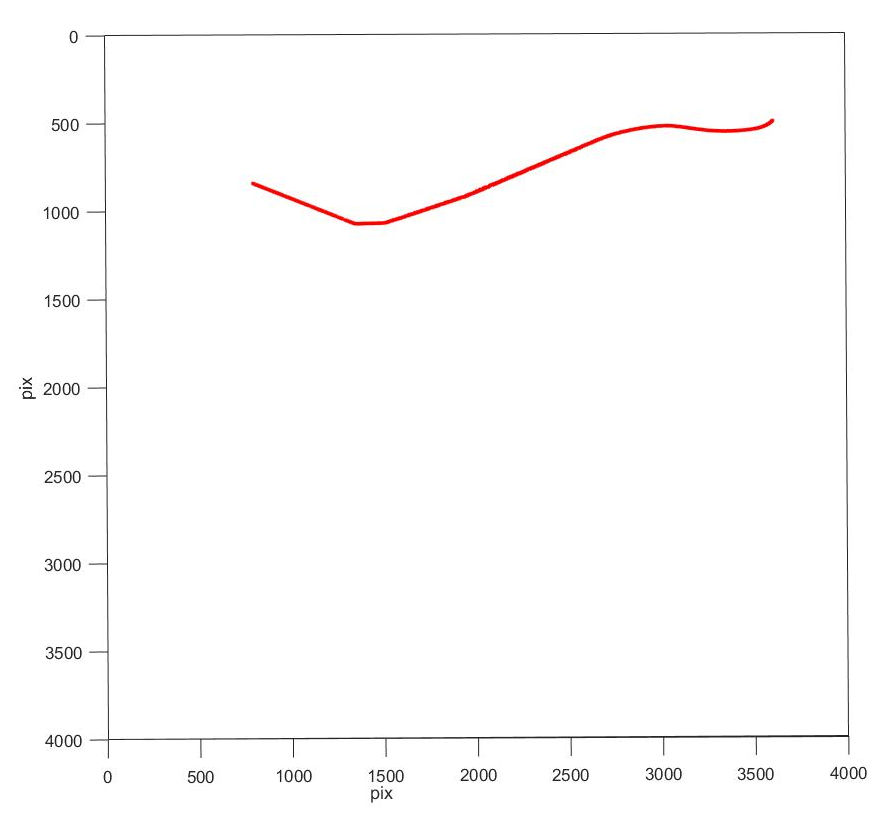
\includegraphics[width=0.9\textwidth]{./images/tech/profile_ex.jpg}
    \end{minipage}
    \caption{Example of profile extraction. On the left there is a live frame of a railway wheel, while, on the right, there is the extracted profile.}
    \label{fig:tech:laser-example}
  \end{figure}
\vfill
  \begin{figure}[t!]
    \centering
    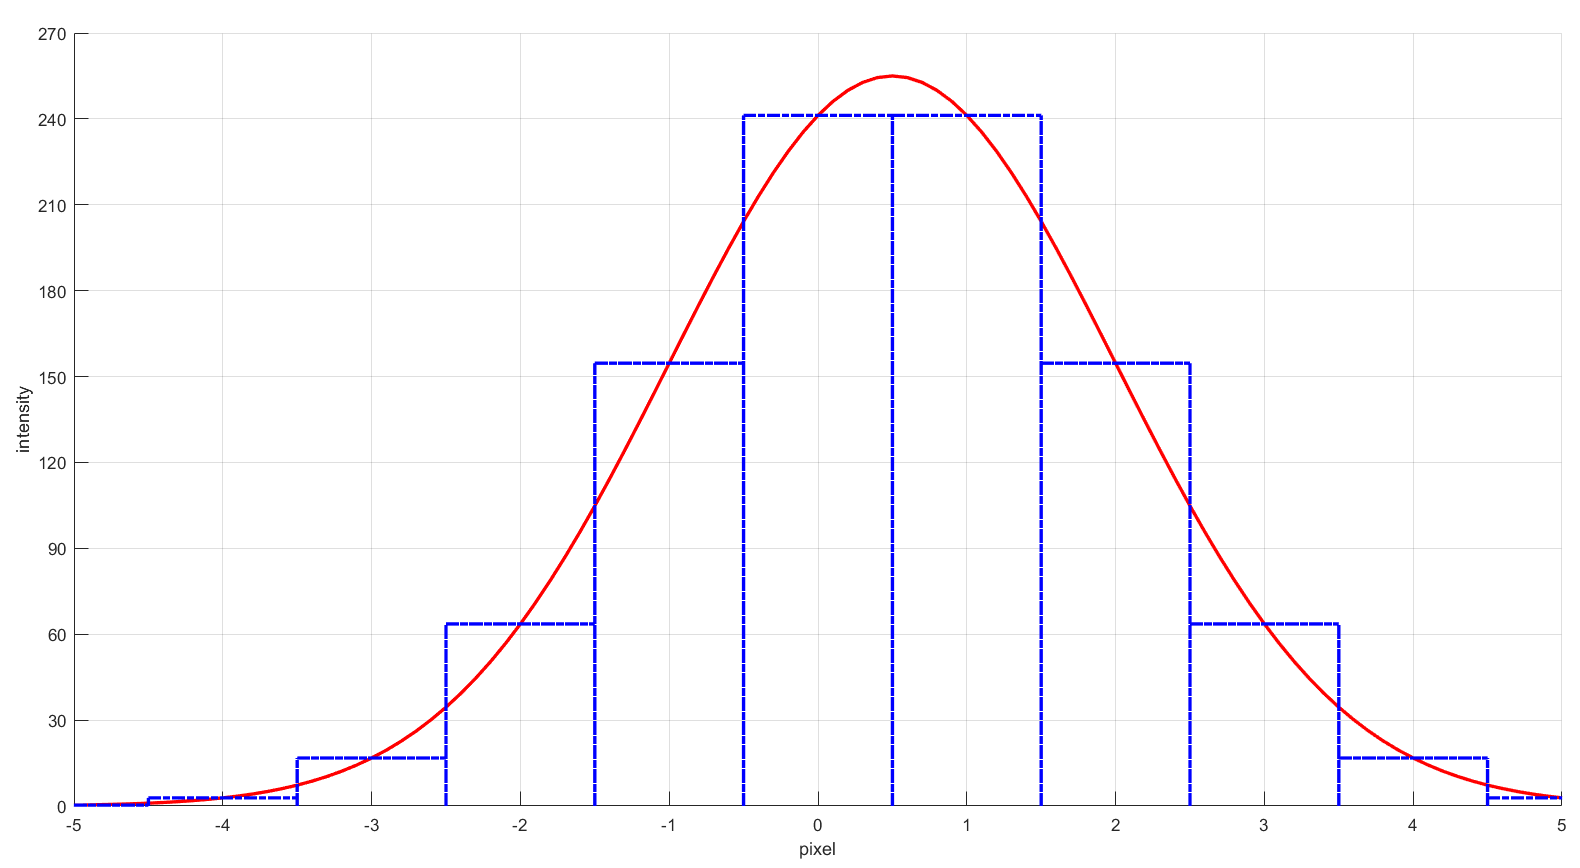
\includegraphics[width=0.79\textwidth]{./images/tech/gauss-discr.png}
    \caption{Gaussian distribution discretization because of pixels.}
    \label{fig:gauss-discr}
  \end{figure}

To try to solve these problems, in literature we can find a lot of solutions, such as in \cite{BLAIS1986145}\cite{Dorsch:94}\cite{1334612}\cite{Naidu1991}\cite{doi:10.1080/095119298130642}.
All of the proposed filters try to approximate the shape of the Gaussian model, starting from the light intensities collected by the pixels, and in this way the peak location with subpixel accuracy is improved. \\
To better understand how these filters works, we grouped them in two categories:
  \begin{itemize}
    \item the first one gathers all that filters that use mathematical relations to fit a Gaussian distribution over the pixels;
    \item the second one gathers all that filters that compute the discrete derivatives of the discrete signal, and use them to locate the global maxima.
  \end{itemize}
Given the pixel collected by the greatest amount of light intensity, all the filters described below locate the peak of the spot using only the pixels along the $y$ axis, consistently with the coordinate reference system used in Section \ref{sec:init-modelanalysis} (parallel to the direction of the laser beam).

In the following of this section, we will indicate with $y$ the coordinates of the pixel candidate to contain the peak of the spot laser, while with $b$ the light intensity collected by that pixel. Then we will indicate with $a$ and $c$ the light intensities collected by the pixels $y-1$ and $y+1$, respectively.

% --------- %
\subsubsection{Centre of Mass (\acs{COM})}
The \acs{COM} (known as \textit{Center of Gravity}, \acs{COG}) is probably the most used subpixel filter. It tries to determine the peak of a gaussian distribution implementing a sliding window mean. Given $a$, $b$ and $c$, we can write:
  \begin{equation}
    \hat{Y} = y +\frac{c - a}{a + b + c}
    \label{eq:sp-com}
  \end{equation}
In literature, it is known that this filter is very sensitive to the noise in the image, in particular it is sensitive to the thermal noise.

% --------- %
\subsubsection{Gaussian approximation}
This filter is based on the idea that the laser spot is similar enough to a Gaussian distribution: as we will see later, this condition is never satisfied because of the thermal noise of the camera. Mathematically, the peak is given by:
  \begin{equation}
    \hat{Y} = y - \frac{1}{2}\left( \frac{\ln{c} - \ln{a}}{\ln{a} - 2\ln{b} + \ln{c}} \right)
    \label{eq:sp-gauss}
  \end{equation}
As we can see, this filter uses only three pixel to determine the position of the peak.

% --------- %
\subsubsection{Linear Interpolation}
Linear interpolation filter simply assumes that a linear relation exists among the usual three points
  \begin{equation}
    \hat{Y} = \begin{cases}
      y - \frac{a - c}{2(b - a)} \qquad if \quad c > a \\
      y - \frac{a - c}{2(b - c)} \qquad otherwise \\
    \end{cases}
    \label{eq:sp-linear}
  \end{equation}

% --------- %
\subsubsection{Parabolic Estimator}
Unlike the previous filter, the parabolic estimator tries to use a continuous vision of the laser signal, so it derives from the Taylor decomposition of the light intensity near the peak.
Let $\delta \in \left[ -\frac{1}{2}, \frac{1}{2} \right]$ be the variation of the peak position with respect to the center of the pixel $y$, and let $f(y + \delta)$ the real value of the peak. Thus, we can write:
  \begin{equation}
  \delta = \frac{f'(y)}{f''(y)} = \frac{f(y+1) - f(y-1)}{2\left( f(y+1) - 2f(y) + f(y+1)\right)}
    \label{eq:sp-parabolic}
  \end{equation}

% --------- %
\subsubsection{Blais and Rioux Detectors}
This filter was originally proposed in \cite{BLAIS1986145}. The original idea was to use a linear interpolator in cascade on a finite impulse asymmetrical digital filter. The authors obtained a linear filter insensitive to laser spot amplitude and, at least theoretically, more robust with respect to the \acs{COM}. Let $f(y)$ be the same function defined for the parabolic estimator, and let $g_d(i)$ a function defined as:
  \begin{equation*}
    g_d(i) = \sum_{k=-d/2}^{-1} f(i + k) - \sum_{k=1}^{d/2} f(i + k)
  \end{equation*}
The estimation of the peak position is given by
  \begin{equation}
      \delta = \frac{g(y)}{g(y) - g(y+1)} 
    \label{eq:sp-br}
  \end{equation}
if $f(y+1) > f(y-1)$; otherwise we will write: $\delta = \frac{g(y-1)}{g(y-1) - g(y)}$.
  
% --------- %
\subsubsection{FIR filter approach}
The last filter we are interested in, is the FIR. As a FIR filter, this one tries to evaluate the discrete derivative of the Gaussian distribution, and looks for the point in which the derivative intersects the origin: that point will be the peak position. We can use the following relation to describe what said so far:
  \begin{equation}
    \hat{Y} = y_0 - \frac{I_0 \cdot \left( y_1 - y_ 0\right)}{I_1 - I_ 0}
    \label{eq:sp-fir}
  \end{equation}
where $I_i$ is the intensity of light collected by the sensor in the pixel; $(y_0, I_0)$ are the coordinate and the intensity of the last point before the origin, while $(y_1, I_1)$ are the coordinate and the intensity of the first point after the origin.

Also in this case, we assume that the error committed locating the peak position is at most half pixel. \\

\bigskip
As we can see, all the filters above are introduced using only three pixels. In real systems this could not be enough to reach a good precision in the measures, generally because of the depths of field of cameras and lasers. Moreover, laser beams can be as thick as $30$ pixels: in these cases, considering only three pixels makes the final approximation very partial, and in saturation conditions the problem is what pixels must be considered. Furthermore, as just mentioned, they are sensitive to the presence of noise in the image. In particular, the thermal noise (described in Subsection \ref{subsec:overview-cameras}) has to be removed before to exploit subpixels optimizations, for example subtracting the background noise of the camera.
Accordingly with \cite{1334612} and \cite{Naidu1991}, Filters \ref{eq:sp-gauss}, \ref{eq:sp-linear}, \ref{eq:sp-parabolic}, \ref{eq:sp-br} and \ref{eq:sp-fir} should be better than \ref{eq:sp-com}, but our analysis shown something different.


% The camera calibration problem
  \section{The camera calibration problem}
\label{sec:teo-calibration}
The \textit{geometric camera calibration} is a process that allows to determine all the parameters introduced with the Equation \ref{eq:perspective_projection}. When we calibrate a single camera, we are determining only its intrinsic parameters, instead if we calibrate a couple of cameras (or, as in this case, a laser-camera pair) we are able to locate the points in the 3D space, and we can determine the extrinsic parameters of the equation. Accordingly with what we said in Subsection \ref{subsec:lenses}, lens distortions are critic when we need to reconstruct the 3D world from an image, so they have to be considered by calibration algorithms that, generally, implement non-linear optimization methods (note that the general model for lens distortions is non-linear). Furthermore, some algorithms (such as \cite{SchCameraCalib} and \cite{hamrouni2012new}) try to consider the distortion due to the lens tilt caused by, in turn, the use of the Scheimpflug principle. \\

In literature there is a multitude of calibration algorithms, most developed for stereocamera systems. In this subsection we briefly introduced two algorithms that can be used to calibrate laser triangulation systems, proposed by Tsai \cite{TsaiTvLenses} (the pioneer of camera calibration algorithms) and Zhang \cite{Zhang-calib}. Both the algorithms are based on the pinhole projective model, described in Equation \ref{eq:perspective_projection}, and take in input a grid of points, both in image and world reference systems, and give in output the camera parameters. As we can understand, the origin of the world reference system could be arbitrary, but the system must be consistent with the world.

The choice of to use these algorithms was done by their interest in our filed of study and by the availability of data to compare. However, the use of non-linear optimizations made it difficult to estimate some parameters of interest for the next analysis.

\subsubsection{Tsai}
Roger Tsai proposed its algorithm in 1987 in order to improve the already existing algorithms, that lacked of many informations, such as lens distortions. Thus, he introduced a two-step process: in the first step he evaluated the intrinsic parameters starting from the grid took in input; in the second step he applied a non-linear optimization to correctly evaluate intrinsic parameters, with particular attention with focal length and lens distortions. As shown in his article, he developed a very accurate, fast and versatile algorithm to calibrate cameras. Furthermore, one of the advantages of this technique is the ability to calibrate using a single planar view of the reference target. \\

As we can read in the Reg Wilson's FAQ\footnote{\url{http://www.ius.cs.cmu.edu/IUS/usrp2/rgw/www/faq.txt}, no longer available now.} we have to be cautious when we set Tsai parameters. First of all, it assumes that some nominal values, such as pixel sizes, sensor size and frame grabber are correct. In this way he simplifies some passages of the algorithm. Second we have to pay attention on the choice of the world reference system: if we consider the coplanar procedure, the origin of our coordinate reference system must to be far from the center of the sensor, otherwise the algorithm could be not work. \\
Both in coplanar and non-coplanar procedure, the input grid must have at least $11$ point to calibrate correctly. Furthermore, the points have to be taken broadly across the \acs{FOV} to let the non-linear optimization work properly. \\

Note that, in order to separate the effects of $f$ and $T_z$ on the image, there needs to be perspective distortion effects in the calibration data. For useable perspective distortion, the distance between the calibration points nearest and farthest from the camera should be on the same scale as the distance between the calibration points and the camera. This applies both to coplanar and non-coplanar calibration:

For co-planar calibration the worst situation is to have the 3D points lied in a plane parallel to the camera's image plane (all points at   equal distance away). Simple geometry tells us we can't separate the effects of $f$ and $T_z$. A relative angle of $30$ degrees or more is recommended to give some effective depth to the data points.

For non-coplanar calibration the worst case is to have the 3D points lied in a volume of space that is relatively small compared to the volume's distance to the camera. From a distance the image formation process is closer to orthographic (not perspective) projection and the calibration problem becomes poorly conditioned.


\subsubsection{Zhang}
Zhang developed an hybrid process that combines self-calibration (a grid similar to that of Tsai) and traditional calibration techniques (match between the same point in different images), which enables the linear estimation of all intrinsic parameters. To do that at least three images of a well known planar pattern (or reasonably considered such) are needed, taken in different positions. The motion of the pattern should not necessarily be known. The steps needed to calibrate the system are the following, to:
  \begin{enumerate}
    \item Print a pattern and attach it to a planar surface.
    \item Take a few images of the model plane under different orientations by moving either the plane or the camera. In the scenarios we are interested in, we will move the pattern keeping fixed the camera.
    \item Detect the feature points in the images.
    \item Estimate the five intrinsic parameters and all the extrinsic parameters using the closed-form solution.
    \item Refine all parameters, including lens distortion parameters.
  \end{enumerate}
Unlike Tsai, Zhang tries to estimate the lens distortions until the fourth degree. As the author admitted in the original paper, his algorithm could degenerate if the pattern took in the different frames, lies in parallel planes.

\bigskip
Now we can understand the importance of planar calibration algorithm in laser-based triangulation systems: the laser forms a flat plane in the 3D world reference system. All points we will acquire lie on this plane. From this point of view, Tsai is preferable with respect to Zhang, because it used a single view of scene, taken on the laser plane. Note that if we use a known pattern (i.e. a checkboard), we must be sure that the pattern lies on the laser plane, otherwise the map that obtained will be incorrect.

  % \clearpage

% 3D computer vision overview
  \section{3D computer vision overview}
The laser-camera triangulation system is not the only way to perform 3D world reconstruction. The most commonly used technologies are:
\begin{itemize}
  \item \textsc{Stereo Vision} - The typical stereo vision system is a binocular system, composed by two cameras displaced horizontally, viewing the same scene at two slightly different angles. Thanks to the epipolar geometry it is possible to determine where a specific 3D world point is projected into the 2D planes of the two cameras. After determining these relations, the relative depth information can be obtained in the form of a disparity map, which encodes the differences in horizontal coordinates of corresponding image points. The values in this disparity map are inversely proportional to the scene depth at the corresponding pixel location.
  
  \item \textsc{Structured light} - Similarly to \acs{SOL} technology, structured light sensors are made by a camera and by a source of light (DLP-projector) that project know patterns, alternating bright and dark. Patterns are deformed because of the shape of the target as with \acs{SOL}, and triangulation is used for the 3D reconstruction. The main benefit of using a DLP-projector rather than a fixed light line is that the projection project the pattern over the whole scene, and mechanical translation or motion required by SOL is not required.

  \item \textsc{Time Of Flight (\acs{TOF})} - This technique is the youngest of the ones proposed. \acs{TOF} sensors estimate distances by measuring the time needed to a signal (light, electromagnetic, acoustic, ...) to reach an obstacle and come back to the sensor. One of the benefits of using this technique is the independence of the calculated distances for each pixel, allowing very high accuracy, but this type of sensors are very delicate and require a lot of handling. \acs{LIDAR} (Light Detection And Ranging) is the first example of \acs{TOF} technology.
  
\end{itemize}
Typically these names are also used to refer to sensors that exploit the specific technology.
